\documentclass{ximera}
%% handout
%% nohints
%% space
%% newpage
%% numbers

%% You can put user macros here
%% However, you cannot make new environments

\graphicspath{{./}{firstExample/}{secondExample/}}

\usepackage{url}
\usepackage{tikz}
\usepackage{tkz-euclide}
\usetkzobj{all}


\tikzstyle geometryDiagrams=[ultra thick,color=blue!50!black]
\pgfplotsset{compat=1.8}
  \usepackage[T1]{fontenc}
  \usepackage[utf8x]{inputenc} %% we can turn off input when making a master document

%\prerequisites{none}


\title{Visualizing Functions}

\begin{document}
\begin{abstract}
We learn three methods for presenting functions: graphing, tables, and formulas.
\end{abstract}
\maketitle

There are three nice methods for presenting a function. We can draw its graph in the plane, create a table, and/or write a formula.

For example, Let $A(x)$ be the the area of the triangle below.
\[
\begin{tikzpicture}
\draw (0,0) --node[below]{$x$} (2,0) -- (0,2) --node[left]{$x$} (0,0) rectangle (.2,.2);
\end{tikzpicture}
\]
\begin{itemize}
\item We can represent $A(x)$ as a table.
\[
\begin{tabular}{cccccccc}
$x$ & $0$ & $1$ & $2$ & $3$ & $4$ & $5$ & $6$\\ \hline
$A(x)$ & $0$ & $.5$ & $2$ & $4.5$ & $8$ & $12.5$ & $18$
\end{tabular}
\]
\item
We can represent $A(x)$ as a formula. The area of a triangle is one half base times height, so $A(x)=\frac{1}{2}x^2$.
\item We can draw a graph of $y=A(x)$.
\begin{image}
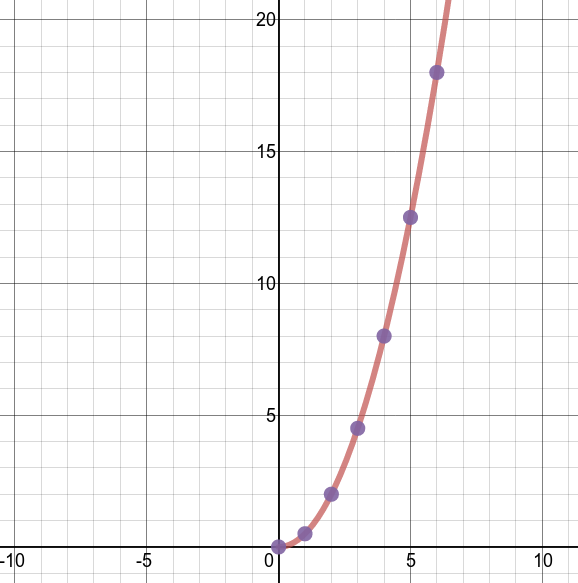
\includegraphics[width=8cm]{TriangleArea.png}
\end{image}
\end{itemize}

All three methods of presenting the function are useful, though some circumstances might make one method more useful than another. The good news is that we will be using a tool to help us obtain these various representations of functions. Watch the video below to learn how to obtain a graph and a table from a function.\youtube{https://www.youtube.com/watch?v=kXgb64qcvik}

\begin{question}
Go to \url{desmos.com} and define the three functions 
\[
f(x)=x^4-2x^3+x^2-x,\quad g(x)=x^5-4x^4+3,\quad\text{and}\quad h(x)=\frac{x^2(x+1)^2}{4}.
\]
Create a table that has $x$-values $-1$, $0$, $1$, $2$, $3$, $4$, and $5$. Create columns with headings $y=f(x)$, $y=g(x)$, and $y=h(x)$.

Now we will compare the output values of each function in our table. For which $x$-values below does the greatest output come from the function $f(x)$?
  \begin{solution}
    \begin{multiple-choice}
      \choice[correct]{$x=-1$}
      \choice{$x=0$}
      \choice{$x=1$}
      \choice{$x=2$}
      \choice{$x=3$}
      \choice[correct]{$x=4$}
      \choice{$x=5$}
    \end{multiple-choice}
    \begin{hint}
    Do the comparison one row at a time.
    \end{hint}    
For which $x$-values below does the greatest output come from the function $h(x)$?
    \begin{multiple-choice}
      \choice{$x=-1$}
      \choice{$x=0$}
      \choice[correct]{$x=1$}
      \choice[correct]{$x=2$}
      \choice[correct]{$x=3$}
      \choice{$x=4$}
      \choice{$x=5$}
    \end{multiple-choice}
    \begin{hint}
    Do the comparison one row at a time.
    \end{hint}
For which $x$-values below does the least output come from the function $g(x)$?
    \begin{multiple-choice}
      \choice[correct]{$x=-1$}
      \choice{$x=0$}
      \choice{$x=1$}
      \choice[correct]{$x=2$}
      \choice[correct]{$x=3$}
      \choice[correct]{$x=4$}
      \choice{$x=5$}
    \end{multiple-choice}
    \begin{hint}
    Negative values are less than positive values. Read the problem carefully.
    \end{hint}
  \end{solution}
\end{question}

\begin{question}
At \url{desmos.com} define a function $f(x)=\sqrt[3]{\frac{1}{x+4}}$. Then find $f(1.6)$ accurate to three decimal places.
\begin{solution}
\begin{hint}
To get a cube root you can use the input panel at the bottom of the screen. Click on the button labeled ``more'' to find additional symbols. 
\end{hint}
$f(1.6)=$ $\answer{0.563}$.
\end{solution}
\end{question}


\end{document}
